\documentclass{article}[11pt]
\usepackage[frenchb,english]{babel}
\usepackage[T1]{fontenc}
\usepackage[utf8]{inputenc}
\usepackage{amsmath,amssymb,latexsym}
\usepackage{times}
\usepackage{float}
\usepackage[left=2cm,right=2cm,top=2cm,bottom=2cm]{geometry}
\frenchbsetup{StandardLists=true} % � inclure si on utilise \usepackage[french]{babel}
\usepackage{enumitem}
\usepackage{fancyhdr}
\usepackage{mathrsfs}
\usepackage{graphicx}
%\usepackage[Algorithme]{algorithm}
%\usepackage{algorithmic}
\usepackage{tikz}
\usepackage{tabularx}
\usetikzlibrary{shapes}
\pagestyle{fancy}
\newcommand{\tr}[1]{{\vphantom{#1}}^{\mathit t}{#1}} 
\renewcommand\headrulewidth{1pt}
\fancyhead[L]{Cours 1�re S}
\fancyhead[R]{Yoann Pietri}
\newcounter{theoremecounter}[subsection]
\usepackage{titlesec}
\setcounter{secnumdepth}{3}% enl�ve la num�rotation apr�s les sections
%\renewcommand\thechapter {\Roman{chapter}}

 \setlength{\parindent}{0pt}

\newcommand{\R}{\mathbb{R}}
\newcommand{\N}{\mathbb{N}}
\newcommand{\Q}{\mathbb{Q}}
\newcommand{\Z}{\mathbb{Z}}
\newcommand{\C}{\mathbb{C}}
\newcommand{\K}{\mathbb{K}}
\newcommand{\eqi}{\Leftrightarrow}
\titleformat{\subsubsection}
   {\normalfont\fontsize{11pt}{13pt}\selectfont\bfseries}% apparence commune au titre et au num�ro
   {\thesubsubsection}% apparence du num�ro
   {1em}% espacement num�ro/texte
   {}% apparence du titre

\tikzstyle{theobox} = [draw=black, very thick,
    rectangle, rounded corners, inner sep=10pt, inner ysep=20pt]
\tikzstyle{theotitle} =[fill=white, text=black,rounded corners,draw=black,very thick]

\fancyhead[L]{Contrôle chapitre 3}

\usepackage{tkz-tab}

\begin{document}
\center
\Large Contrôle de cours (correction)
\flushleft
\center
Dérivation
\flushleft \normalsize
\subsection*{Exercice 1 (R.O.C., temps conseillé : 10 min) : }
On dit qu'une fonction $f$ est dérivable en $a$ si $$\underset{h\rightarrow 0}{\lim} \frac{f(a+h) - f(h)}{h}$$ Le cas échant on note $$f'(a) = \underset{h\rightarrow 0}{\lim} \frac{f(a+h) - f(h)}{h}$$. Si $f$ et $g$ sont dérivables sur $I$ alors $f+g$ et $f\times g$ sont dérivables sur $I$ et on a $$(f+g)' = f'+g'$$ $$(f\times g)' = f'g+fg'$$. Si $f$ et $g$ sont dérivables sur $I$ et si $g$ ne s'annule pas sur $I$ alors $\frac{f}{g}$ est dérivable sur $I$ et $$\left(\frac{f}{g}\right)' = \frac{f'g-fg'}{g^2}$$ On a $$a \text{ est un extremum local} \Leftrightarrow f' \text{ s'annule en changeant de signe}$$
\subsection*{Exercice 2 (Calculs de dérivée, temps conseillé : 10 min) : }
Pour les 3 fonctions : donner le domaine de définition et montrer qu'elles sont dérivables sur un ensemble à préciser. Exprimer ensuite la dérivée
\begin{enumerate}
\item $$f:x\mapsto 3x^4+4x^2+3$$
$f$ est définie sur $\R$ et dérivable sur $\R$ comme somme de fonctions dérivables sur $\R$. De plus, pour tout $x \in \R$, $$\boxed{f'(x) = 12x^3 + 8x}$$
\item $$g:x\mapsto \frac{x^3 + \sqrt{x}}{(x+4)^2}$$
$g$ est définie sur $[0,+\infty[$ (racine carrée). De plus $(x+4)^2$ ne s'annule pas sur $[0,+\infty[$. $g$ est dérivable sur $]0,+\infty[$ comme quotient d'une fonction dérivable sur $]0,+\infty[$ et d'une fonction dérivable sur $]0,+\infty[$ qui ne s'annule pas sur $]0,+\infty[$ ($x\mapsto x^3 + \sqrt{x}$ est dérivable sur $]0,+\infty[$ comme somme d'une fonction dérivable sur $\R$ et d'une fonction dérivable sur $]0,+\infty[$). De plus, pour tout $x\in ]0,+\infty[$, on a$$\boxed{g'(x)=\frac{(3x^2 + \frac{1}{2\sqrt{x}})(x+4)^2 + (x^3 + \sqrt{x})(2x+8)}{(x+4)^4}}$$ Pourquoi la dérivée de $x\mapsto (x+4)^2$ ets $x\mapsto 2x+8$ ? Il suffit d'écrire $(x+4)^2 = x^2 + 8x + 16$ d'après les identités remarquables et de dériver
\item $$h:x\mapsto \sqrt{x^2-2x+1}$$ sur $[1,+\infty[$\newline
Pour tout $x\in \R$, 
$$x^2-2x+1 = (x-1)^2$$ 
ainsi sur $[1,+\infty[$
$$\sqrt{x^2-2x+1} = x-1$$ donc est dérivable de dérivée $x\mapsto 1$
\end{enumerate}
\subsection*{Exercice 3 (Etude de deux fonctions, temps conseillé : 20 min) : }
\begin{enumerate}
\item $f$ est une fonction trinôme donc définie sur $\R$
\item $f$ est dérivable sur $\R$ comme somme de fonctions dérivables sur $\R$
\item On a pour tout $x\in \R$, 
$$f'(x) = 3x^2 - 2\times \frac{3}{2}x -6$$
$$\boxed{f'(x) = 3x^2 - 3x - 6}$$
\item On calcule les racines de $f'$ : $$\Delta  = 3^2 + 4\times 3\times6 = 81$$ $\Delta > 0$ donc ce trinôme admet deux racines réelles distinctes qui sont 
$$x_1 = \frac{3 - \sqrt{81}}{2\times 3} = \frac{3-9}{6}$$
$$\boxed{x_1 = -1}$$
$$x_2 = \frac{3 + \sqrt{81}}{2\times 3} = \frac{3+9}{6}$$
$$\boxed{x_1 = 2}$$
Le coefficient dominant du trinôme étant positif, le trinôme est négatif entre les racines. Le tableau de signe est donné à la question suivante avec le tableau de variation de $f$
\item Tableau de signe et de variation \newline
\begin{tikzpicture}
   \tkzTabInit{$x$ / 1 , $f'(x)$ / 1, $f(x)$ / 1.5}{$-\infty$, $-1$,$2$, $+\infty$}
   \tkzTabLine{, +, z, -,z,+ }
   \tkzTabVar{-/, +/$f(-1)$, -/$f(2)$, +/}
\end{tikzpicture}
\item $f'$ s'annule en changeant de signe en $x=-1$ et $x=2$. Ainsi les extrémaux de $f$ sont $f(-1)$ et $f(2)$ avec $$\boxed{f(-1) = \frac{11}{2}}$$ et $$\boxed{f(2) = -8}$$ Pour être plus précis, on peut dire que $f(-1)$ est un maximum local de $f$ et $f(2)$ un minimum local. NB : on aurait pu indiquer $\frac{11}{2}$ et $-8$ directement dans le tableau de signe/variation
\item On trace la courbe représentative de $f$ : \newline
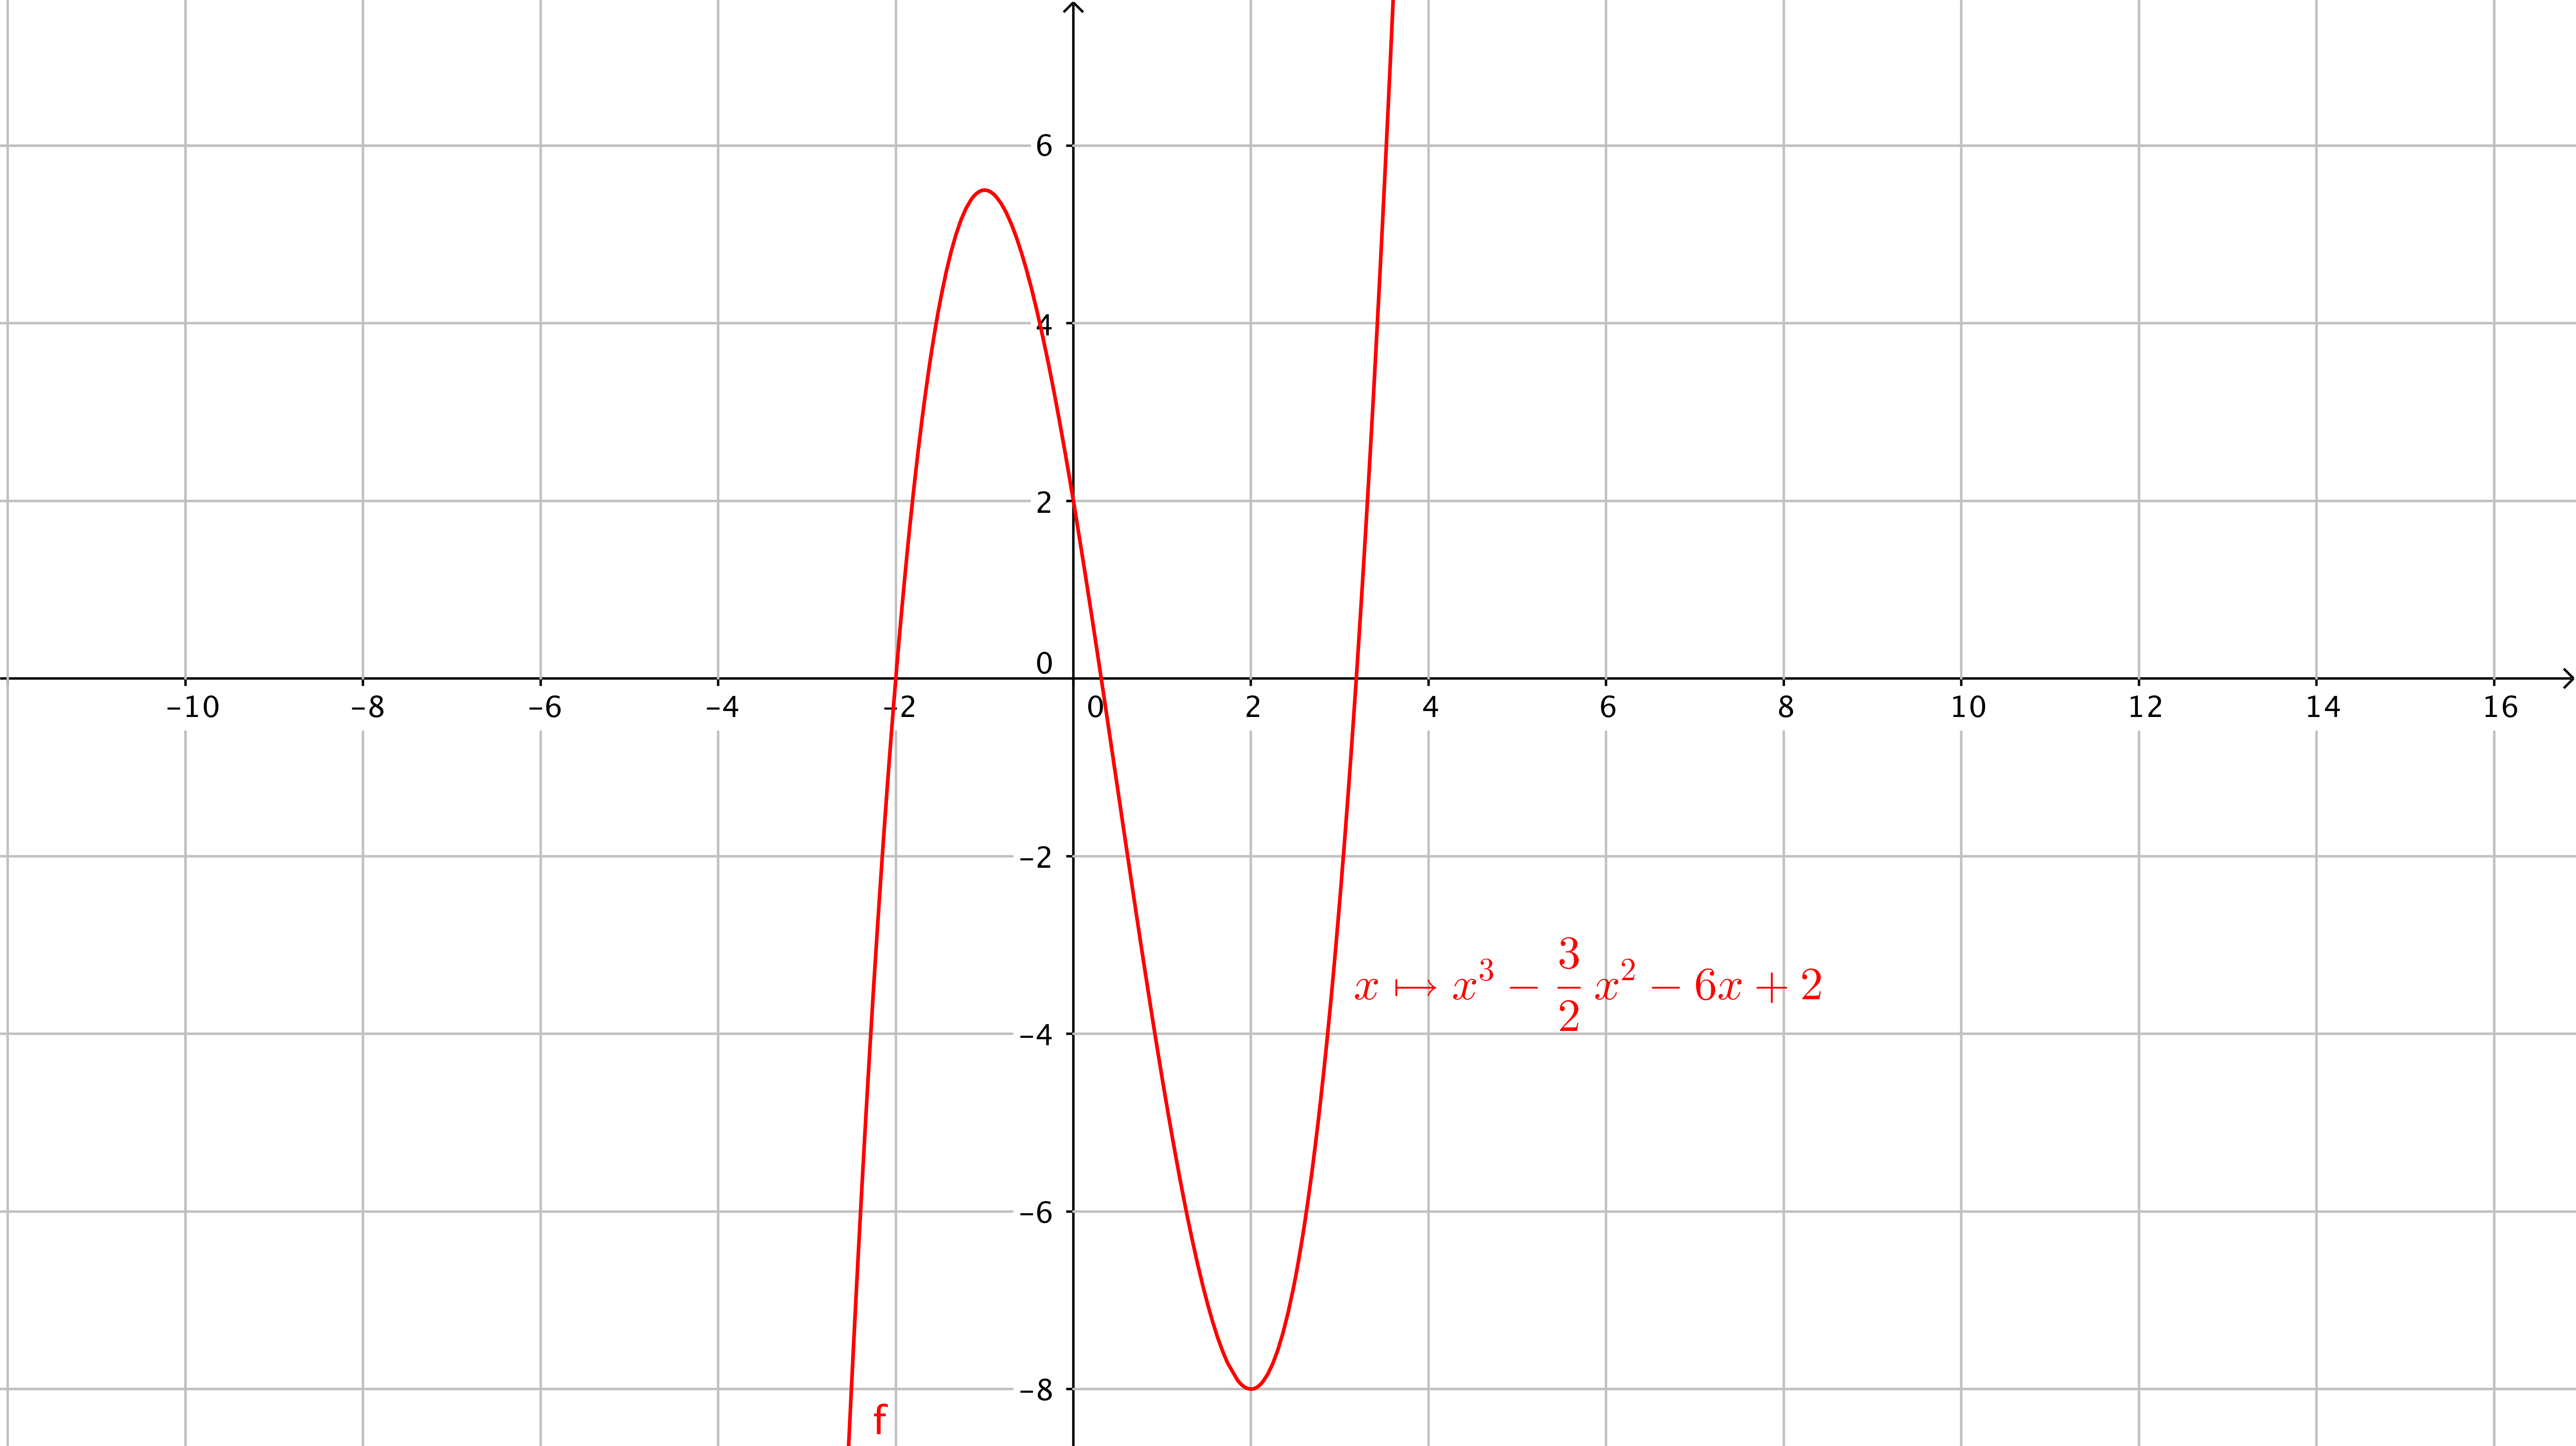
\includegraphics[scale=0.5]{chap3_corr_ill1.png}
\item Pour tout $x\in\R$, $x^2+1 > 0$ donc $g$ est définie sur $\R$
\item On va (évidement !) utiliser la dérivée de $g$ puisque $g$ est dérivable sur $\R$ comme inverse d'une fonction dérivable sur $\R$ qui ne s'annule pas sur $\R$. De plus, pour tout $x\in \R$, 
$$g(x) = - \frac{2x}{(x^2+1)^2}$$
On a $$g(x) = 0 \Leftrightarrow x=0$$ et $$g(x) > 0 \Leftrightarrow x<0$$
Ainsi, on peut déduire le tableau de signe variation : \newline
\begin{tikzpicture}
   \tkzTabInit{$x$ / 1 , $g'(x)$ / 1, $g(x)$ / 1.5}{$-\infty$, $0$, $+\infty$}
   \tkzTabLine{, +,z,- }
   \tkzTabVar{-/, +/$g(0)$,-/}
\end{tikzpicture}\newline
On trouve par la même occasion un maximum local (même global d'ailleurs) atteint en 0 : $g(0)=1$ (g' s'annule en changeant de signe en 0)
\end{enumerate}
\subsection*{Exercice 4 (Tableau de variation d'un trinôme, temps conseillé : 20 min) : }
\begin{enumerate}
\item $f$ est définie est dérivable sur $\R$ comme somme de fonctions dérivables. On a de plus pour tout $x\in \R$, 
$$\boxed{f'(x) = 2ax+b}$$ qui est une \textbf{fonction affine}
\item Dans tous les cas 
$$f'(x) = 0 \Leftrightarrow x = -\frac{b}{2a}$$
\underline{1er cas : $a > 0$}\newline
Dans ce cas, on a $$f'(x) > 0 \Leftrightarrow x > -\frac{b}{2a}$$ et on déduit le tableau de signe/variation \newline
\begin{tikzpicture}
   \tkzTabInit{$x$ / 1 , $f'(x)$ / 1, $f(x)$ / 1.5}{$-\infty$, $-\frac{b}{2a}$, $+\infty$}
   \tkzTabLine{, -,z,+}
   \tkzTabVar{+/, -/$f\left(-\frac{b}{2a}\right)$,+/}
\end{tikzpicture}\newline
\underline{2ème cas : $a < 0$}\newline
Dans ce cas, on a $$f'(x) > 0 \Leftrightarrow x < -\frac{b}{2a}$$ (on inverse le sens de l'inégalité car on divise par un nombre négatif) et on déduit le tableau de signe/variation \newline
\begin{tikzpicture}
   \tkzTabInit{$x$ / 1 , $f'(x)$ / 1, $f(x)$ / 1.5}{$-\infty$, $-\frac{b}{2a}$, $+\infty$}
   \tkzTabLine{, +,z,-}
   \tkzTabVar{-/, +/$f\left(-\frac{b}{2a}\right)$,-/}
\end{tikzpicture}\newline
\item Dans tous les cas, la dérivée s'annule bien en changeant dans signe en $\displaystyle x=-\frac{b}{2a}$ et le fait que ce soit un maximum ou un minimum, il suffit de regarder les variations de $f$ selon le signe de $f$
\end{enumerate}
$$\star \star \star$$
\center
FIN DU SUJET
\end{document}